% 5.1.      Propiedades giroscópicas aplicadas al instrumental aeronáutico de a bordo.
% Version 2019

\section{Propiedades del gir\'oscopo}
\label{sec:propiedades.giroscopo}

\begin{frame}{Un poco de historia...}
  
  \begin{columns}
    \begin{column}{0.3\textwidth}
      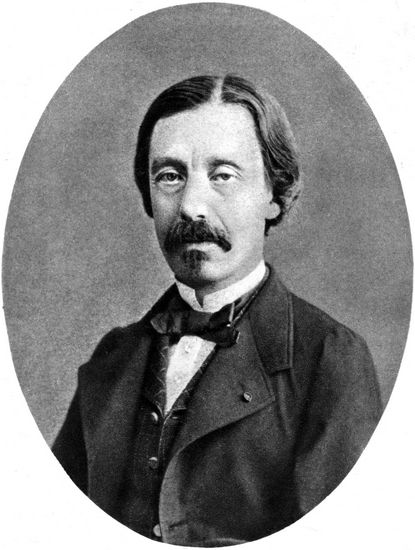
\includegraphics[width=0.7\linewidth]{05.instrumentos.giroscopicos.imagenes/05.01.movimientos/foucault.jpg}

      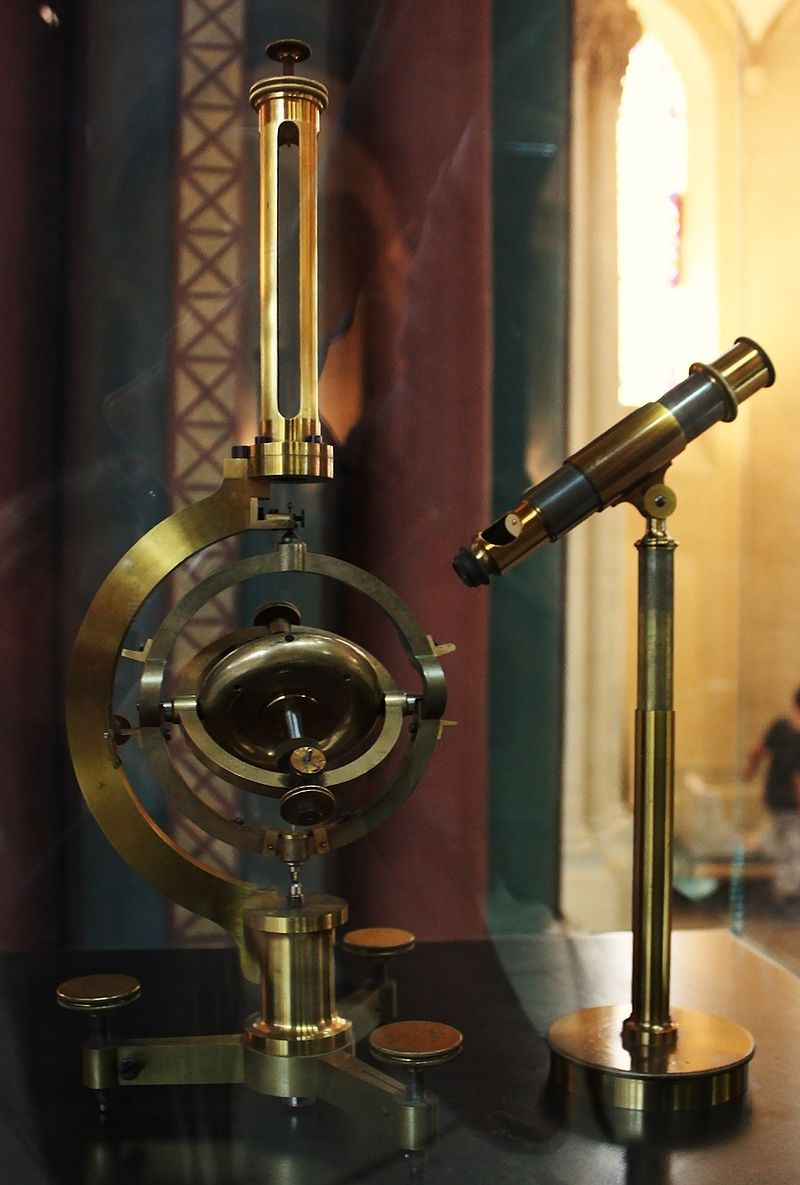
\includegraphics[width=0.7\linewidth]{05.instrumentos.giroscopicos.imagenes/05.01.movimientos/foucault_giroscopo_wiki.jpg}\\
      {\tiny Fuente: Wikipedia}
    \end{column}
    \begin{column}{0.7\textwidth}{\small

  \begin{block}{Etimolog\'ia}
    Gir\'oscopo proviene del griego,
	{\it gyros}: rotaci\'on y {\it skopein}: vista/
  \end{block}

      \begin{exampleblock}{Desarrollo del gir\'oscopo}
        Bernard Le\'on Foucault (1819-1868) invent\'o el gir\'oscopo
        en 1852 y le permiti\'o observar el giro del planeta Tierra.
        Mont\'o una masa rotatoria en un soporte de Cardano para un
        experimento que demostrara la rotaci\'on de la Tierra.  Aunque
        ya hab\'ia demostrado la rotaci\'on de este cuerpo con el
        p\'endulo que lleva su nombre, no comprend\'ia por qu\'e la
        velocidad de rotaci\'on del mismo resultaba m\'as lenta que la
        velocidad de rotaci\'on de la Tierra por un factor
        $\sin{\lambda}$, donde $\lambda$ representa la latitud donde
        se encuentra el p\'endulo.  Por lo anterior, Foucault se di\'o
        cuenta que necesitaba otro aparato para demostrar la
        rotaci\'on de la Tierra de forma m\'as simple y utiliz\'o los
        trabajos del astr\'onomo alem\'an Johann Bohnenberger.
      \end{exampleblock}
	}
    \end{column}
  \end{columns}
  
\end{frame}

\begin{frame}{El gir\'oscopo}

      \begin{columns}
        \begin{column}{0.2\textwidth} \centering

% \animategraphics[loop,width=\linewidth]{10}{05.instrumentos.giroscopicos.imagenes/05.01.movimientos/05.01.giroscopo.animado/giroscopo_animado-}{0}{59}


% \animategraphics[loop,width=\linewidth]{10}{05.instrumentos.giroscopicos.imagenes/05.01.movimientos/05.01.gimbal/gimbal-}{0}{99}

          
        \end{column}
      \begin{column}{0.8\textwidth}
      Un gir\'oscopo consiste en una masa rotante, con forma de rueda, 
	cuyo eje se sujeta a una armaz\'on o cuna (gimbal) 
	interior y \'esta a otra cuna exterior. Este sistema se encuentra libre de rotar en el espacio.

      El gir\'oscopo posee las siguientes propiedades:
      \begin{enumerate}
      \item {\bf Rigidez:} es la que permite que rote siempre en el mismo plano y se opone a cualquier momento
	 que tienda a cambiarlo.
      \item {\bf Precesi\'on:} consiste en la variaci\'on angular del plano de rotaci\'on bajo el influjo 
      de la aplicaci\'on de un momento. Su valor es proporcional a la intensidad del momento aplicado e 
      inversamente proporcional al momento de inercia y momento cin\'etico del rotor.
      \end{enumerate}
    \end{column}
    \end{columns}

	\vspace{0.3cm}
% {\tiny Animaci\'on de un conjunto de tres ejes. Fuente: Lars H. Rohwedder (User:RokerHRO) - Trabajo propio,
%  Dominio p\'ublico, \url{https://es.wikipedia.org/wiki/Suspensi\%C3\%B3n_card\%C3\%A1n#/media/Archivo:Rotating_gimbal-xyz.gif}
% }

%      {\tiny Imagen Suspensi\'on Cardan. Fuente: De Lars H. Rohwedder (User:RokerHRO) - Trabajo propio, 
%      Dominio p\'ublico, \url{https://commons.wikimedia.org/w/index.php?curid=1352775}}

  \href{https://www.youtube.com/watch?v=JnKloSdUJLo}{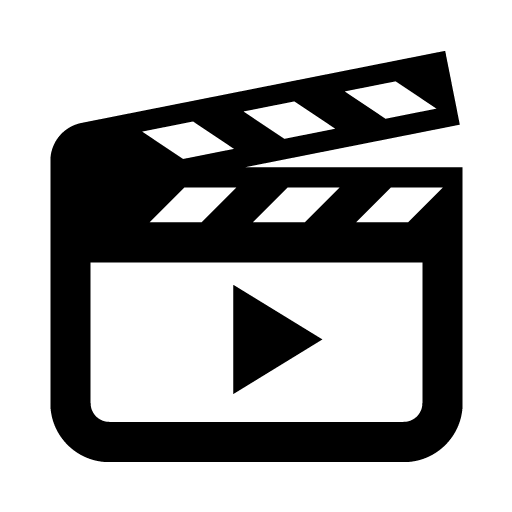
\includegraphics[width=0.1\textwidth]{05.IyA.imagenes/Video.png}}\,Instrumentos girosc\'opicos

\end{frame}

%----------------------Aplicaciones giroscopo
\begin{frame}{Aplicaciones gir\'oscopo}
  \begin{itemize}
  \item Gir\'oscopos libres
    \begin{itemize}
    \item Ejemplo: sistemas inerciales
    \end{itemize}
  \item Gir\'oscopos de desplazamiento
    \begin{itemize}
    \item Dos (2) grados de libertad
    \item Detecta desplazamientos angulares
    \item Utililiza la propiedad de rigidez
    \item Como referencia direccional se emplea uno de eje horizontal
    \item Como referencia en cabeceo y alabeo se emplea uno de eje vertical
    \item Ejemplos: horizonte artificial, comp\'as girosc\'opico
    \end{itemize}
  \item Gir\'oscopos de velocidad
    \begin{itemize}
    \item Un (1) grado de libertad
    \item Detecta velocidades angulares
    \item utiliza la propiedad de precesi\'on
    \item Ejemplo: indicador de giro y viraje
    \end{itemize}

  \end{itemize}
\end{frame}

\begin{frame}{Accionamiento del gir\'oscopo}

  \begin{itemize}
  \item
    \href{https://www.youtube.com/watch?v=q2Zgvxn4rSA}{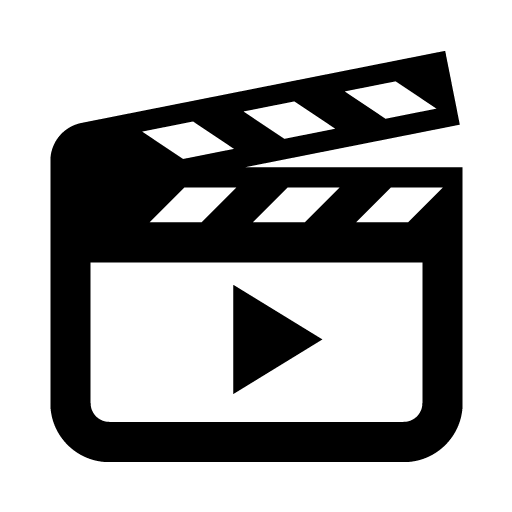
\includegraphics[width=0.1\textwidth]{05.IyA.imagenes/Video.png}}\,
    Gir\'oscopo neum\'atico

  \item     \href{https://www.youtube.com/watch?v=FYSHEhksBjk}{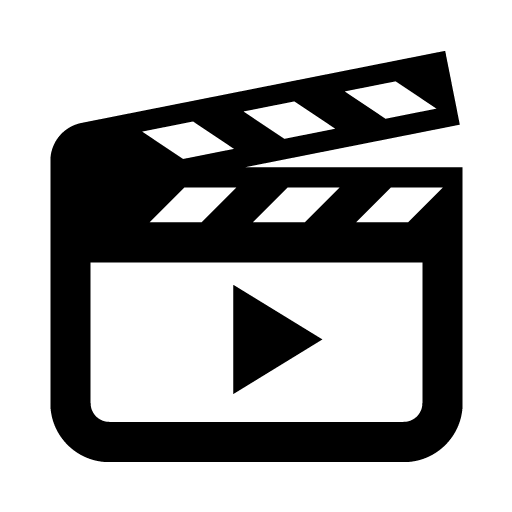
\includegraphics[width=0.1\textwidth]{05.IyA.imagenes/Video.png}}\, 
 \href{https://www.youtube.com/watch?v=VycrS3VYjeM}{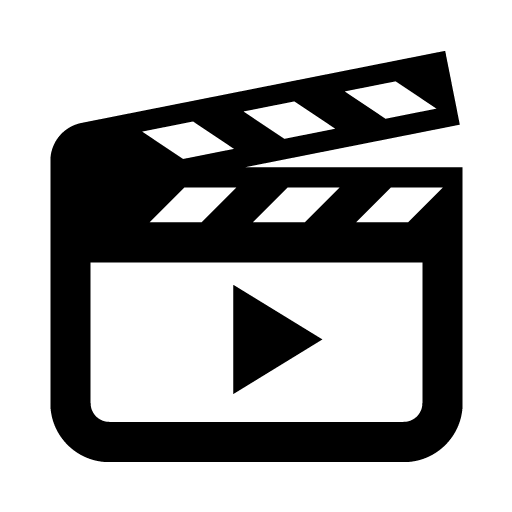
\includegraphics[width=0.1\textwidth]{05.IyA.imagenes/Video.png}}
\, Gir\'oscopo el\'ectrico

\item \href{https://www.youtube.com/watch?v=8IYkisyOZvs}{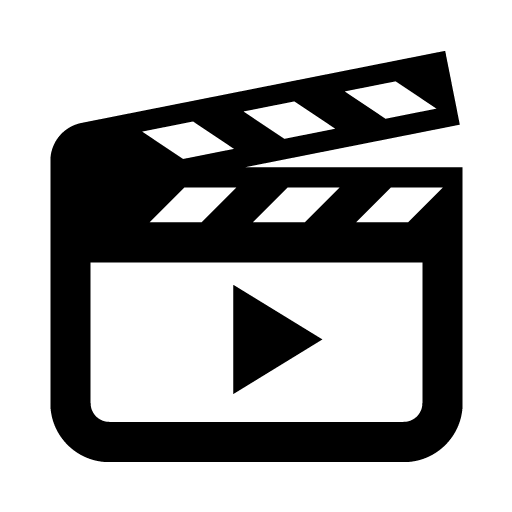
\includegraphics[width=0.1\textwidth]{05.IyA.imagenes/Video.png}}\, Gir\'oscopo laser

\item \href{https://www.youtube.com/watch?v=z62CxCSRMjY}{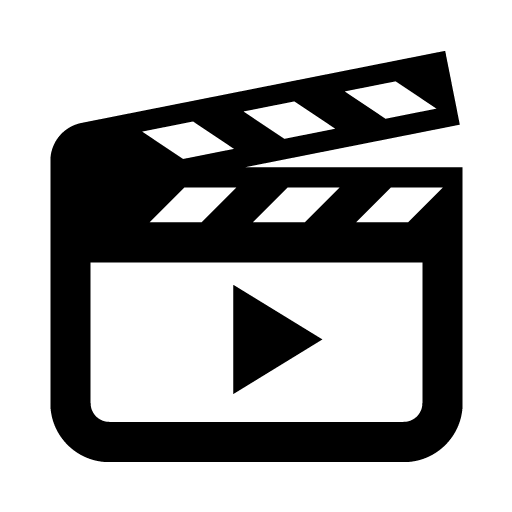
\includegraphics[width=0.1\textwidth]{05.IyA.imagenes/Video.png}}\, Gir\'oscopo de fibra \'optica

  \end{itemize}

\end{frame}


